\documentclass[../Article_Model_Parameters.tex]{subfiles}
\graphicspath{{\subfix{../Figures/}}}
\begin{document}
	
	\label{CH: Results}
	
	The sensitivity equations were solved simultaneously with the original process model. The focus of this work is to investigate the influence of inlet temperature, pressure and mass flow-rate on the state-space as wall as on the extraction yield. The process model and parameters have been discussed in {\color{red}article 1}. The process model was calibrated on set of experiments obtained at different operating conditions, $40^\circ C$ - $50^\circ C$ and 200 bar - 300 bar. The sensitivity analysis has been performed under assumption that the system operates are $45^\circ C$, 250 bar, 0.4 l/min and the simulation was performed with the time step of 0.01 [min].
	
	\subsection{Flow-rate}
	
	The increase of the mass-flow rate affects the whole system simultaneously in the spatial direction. The change in mass flow-rate makes the fluid moves faster, but its thermodynamic state is not affected. \todo{Change the description} As the result, Figure \ref{fig:Sensitivty_F_P} show no change in pressure during the simulation. 
    
    \begin{figure}[h!]
    	\centering
    	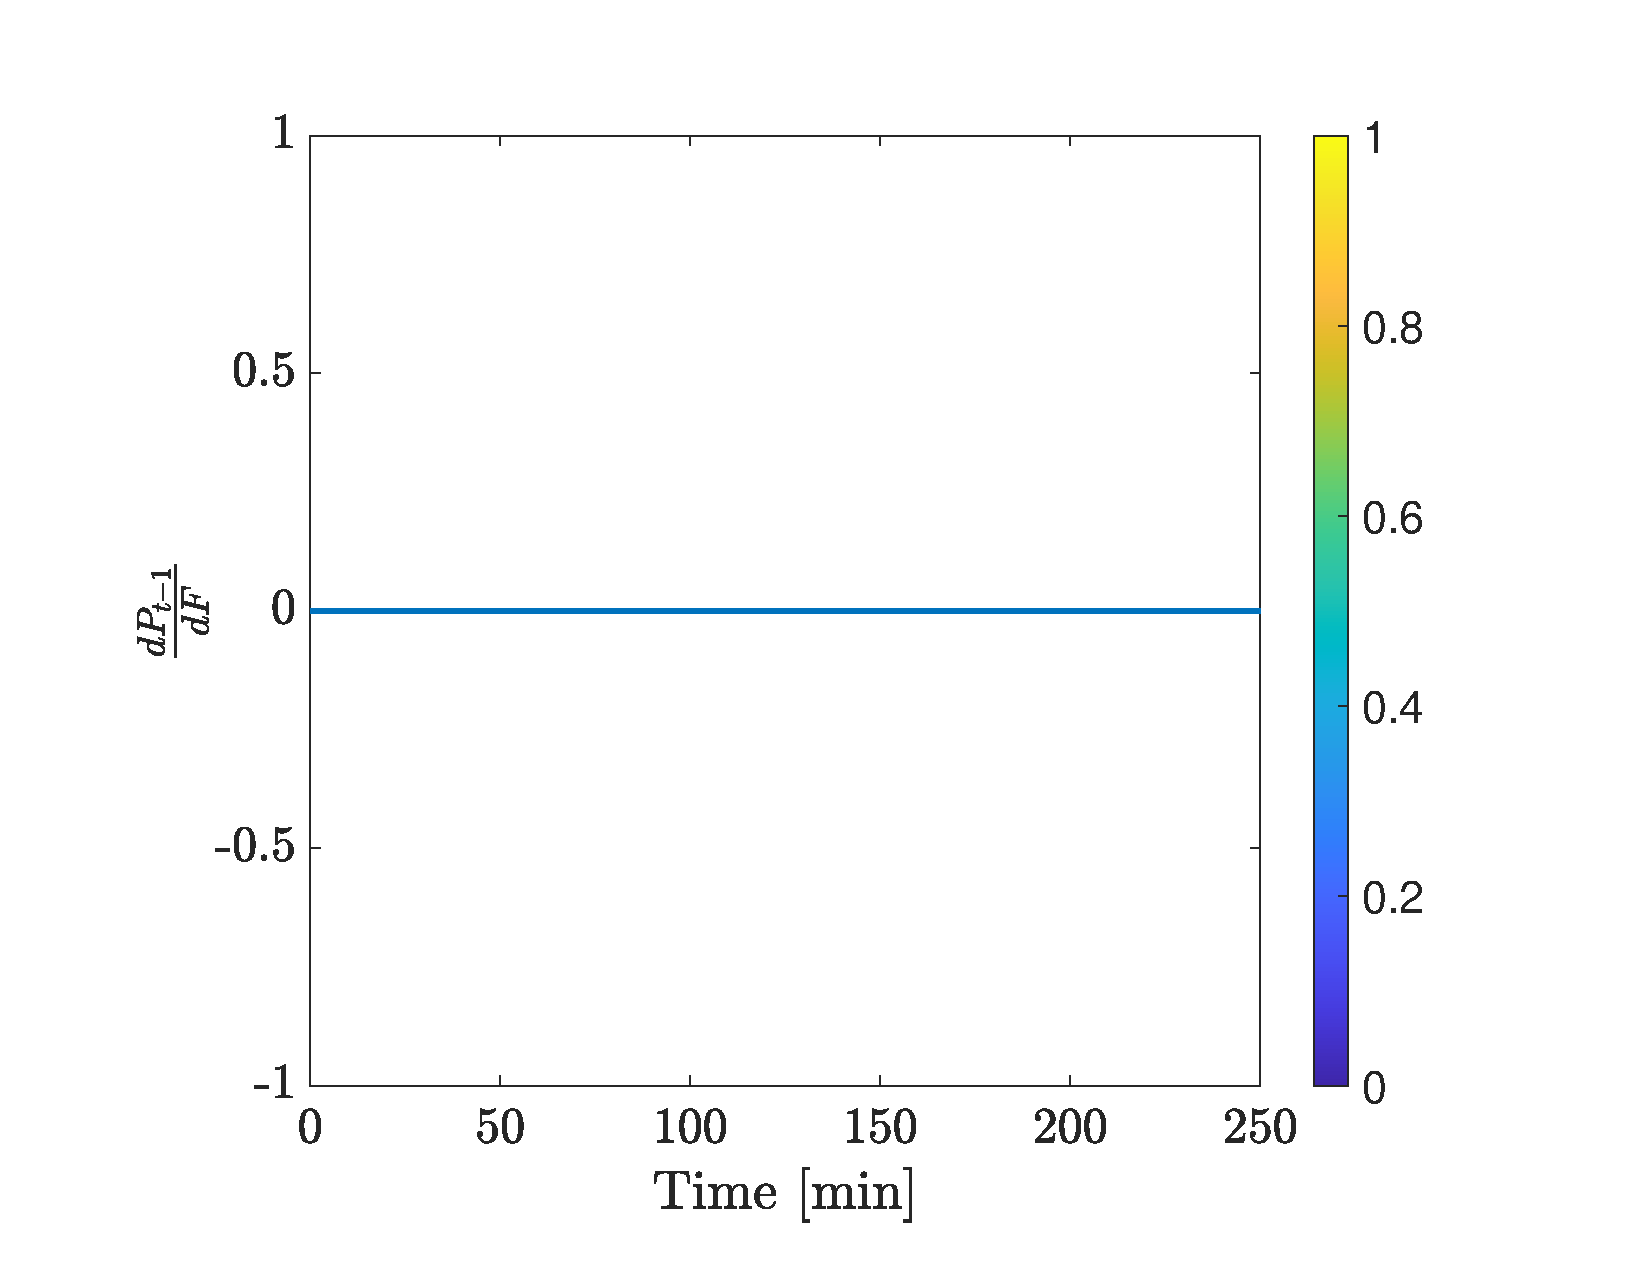
\includegraphics[trim = 1.5cm 1cm 0.5cm 1.0cm,clip,width=\columnwidth]{/Results_sensitivity/P_F.pdf}
    	\caption{The effect of $F$ change on $P$}
    	\label{fig:Sensitivty_F_P}
    \end{figure}
    
    Similarly, the energy in the system (defined as $\rho \times h$) is not affected as presented on Figure \ref{fig:Sensitivty_F_H}. As pressure and temperature are not affected by the increase in the mass flow-rate, the fluid density $\rho$ and enthalpy $h$ are insensitive to flow-rate change. \todo{Change the description}
    
    \begin{figure}[h!]
    	\centering
    	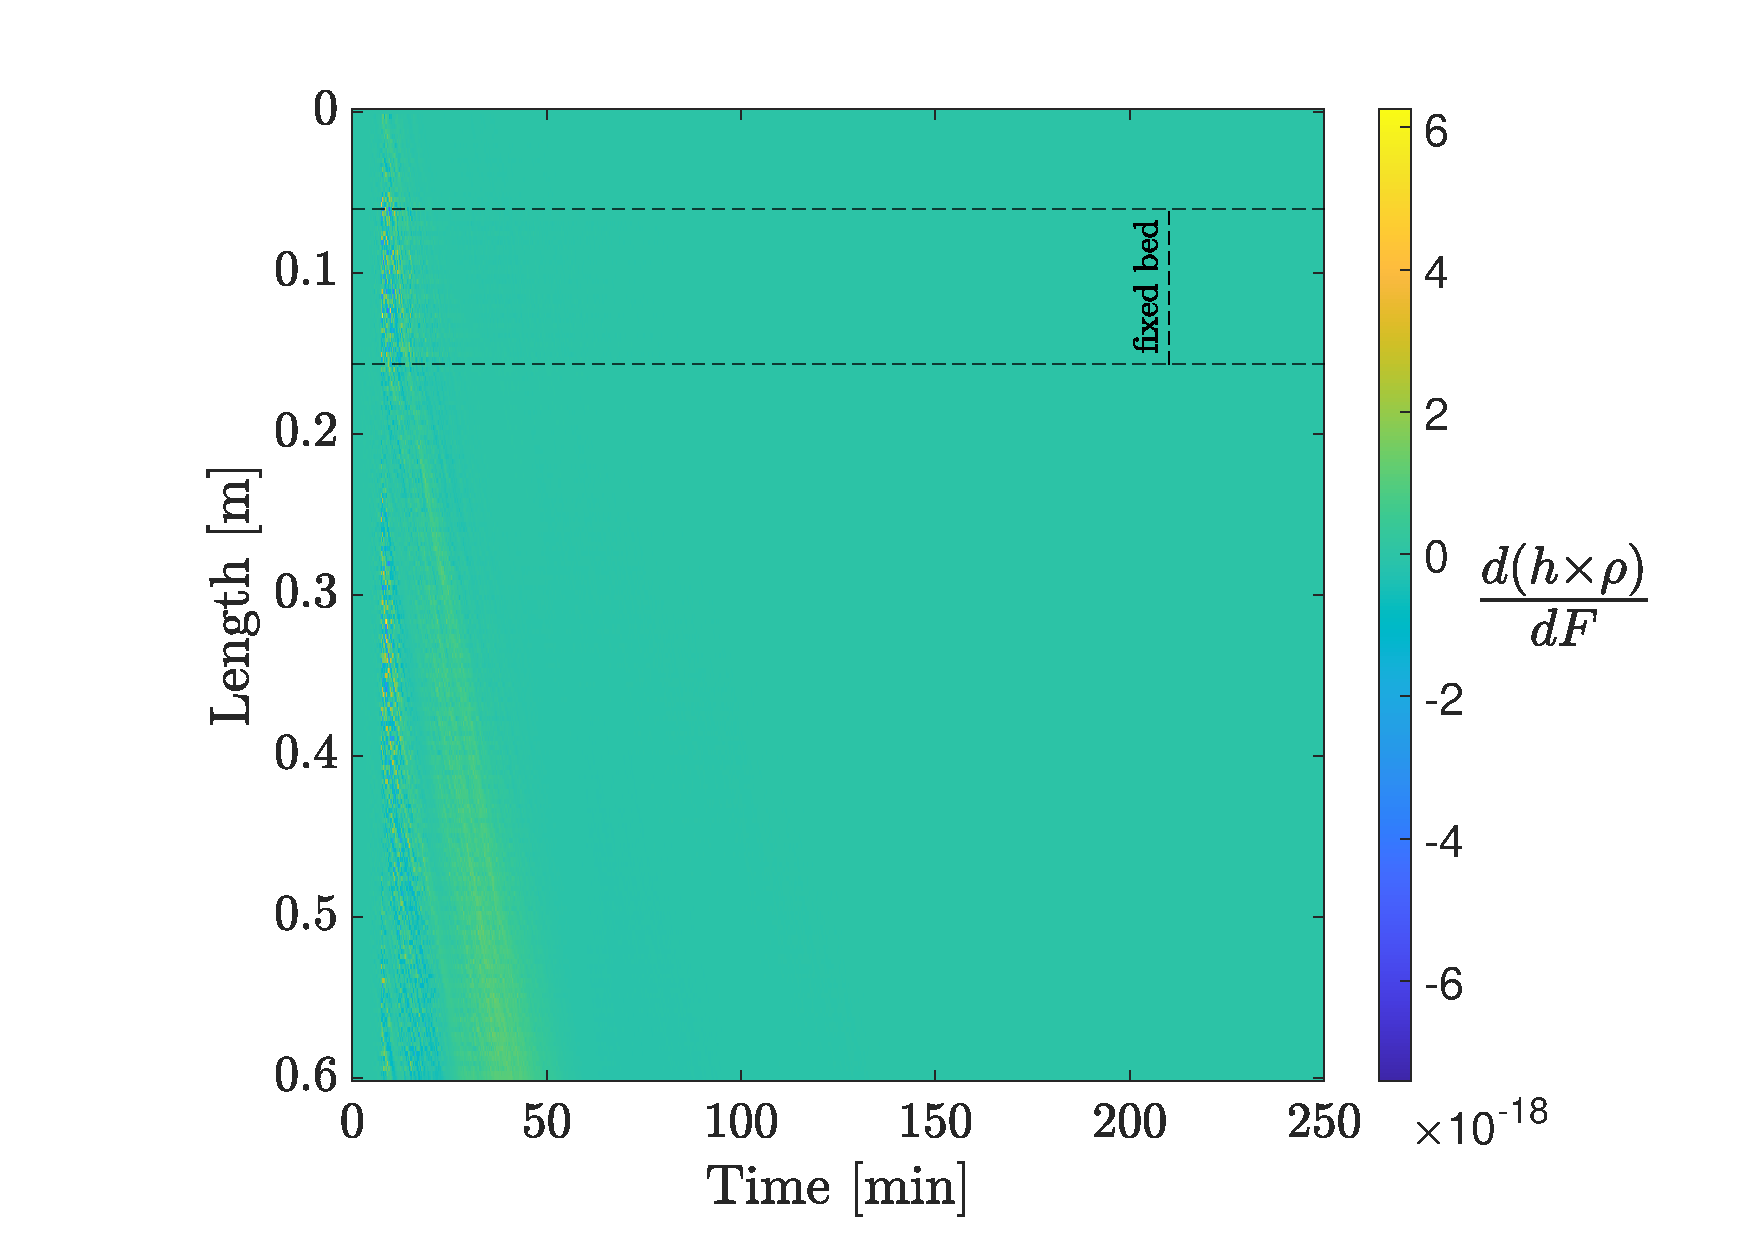
\includegraphics[trim = 1.5cm 1cm 0.5cm 1.0cm,clip,width=\columnwidth]{/Results_sensitivity/H_F.pdf}
    	\caption{The effect of $F$ change on $\rho \times h$}
    	\label{fig:Sensitivty_F_H}
    \end{figure}
    
    The increase in the mass flow rate affects the concentration gradient and accelerates the extraction kinetics. Negative sensitivities in Figure \ref{fig:Sensitivty_F_CS} present the faster extraction rate. Negative values of $dc_s/dF$ can be interpreted as a 'faster' mass loss from the solid phase, which means the extraction efficiency improves. At the beginning of the extraction process, the change in the flow rate has a minimal effect on the extraction process (represented by close to zero sensitivities), due to the high concentration gradient, which leads the extraction kinetic. Later, the increment of the mass flow rate accelerates the extraction kinetic and sensitivities along the decrease to minimum values. Over time, the amount of solute in the solid phase decreases, and eventually, the extraction kinetic becomes limited by the concentration gradient. This behaviour is represented by sensitivities, which asymptotically go to zero. The asymptotic movement of sensitivities can be explained by the fact that the increase in the flow rate does not affect the extraction if all the solute has been removed from the solid phase.
    
    \begin{figure}[h!]
    	\centering
    	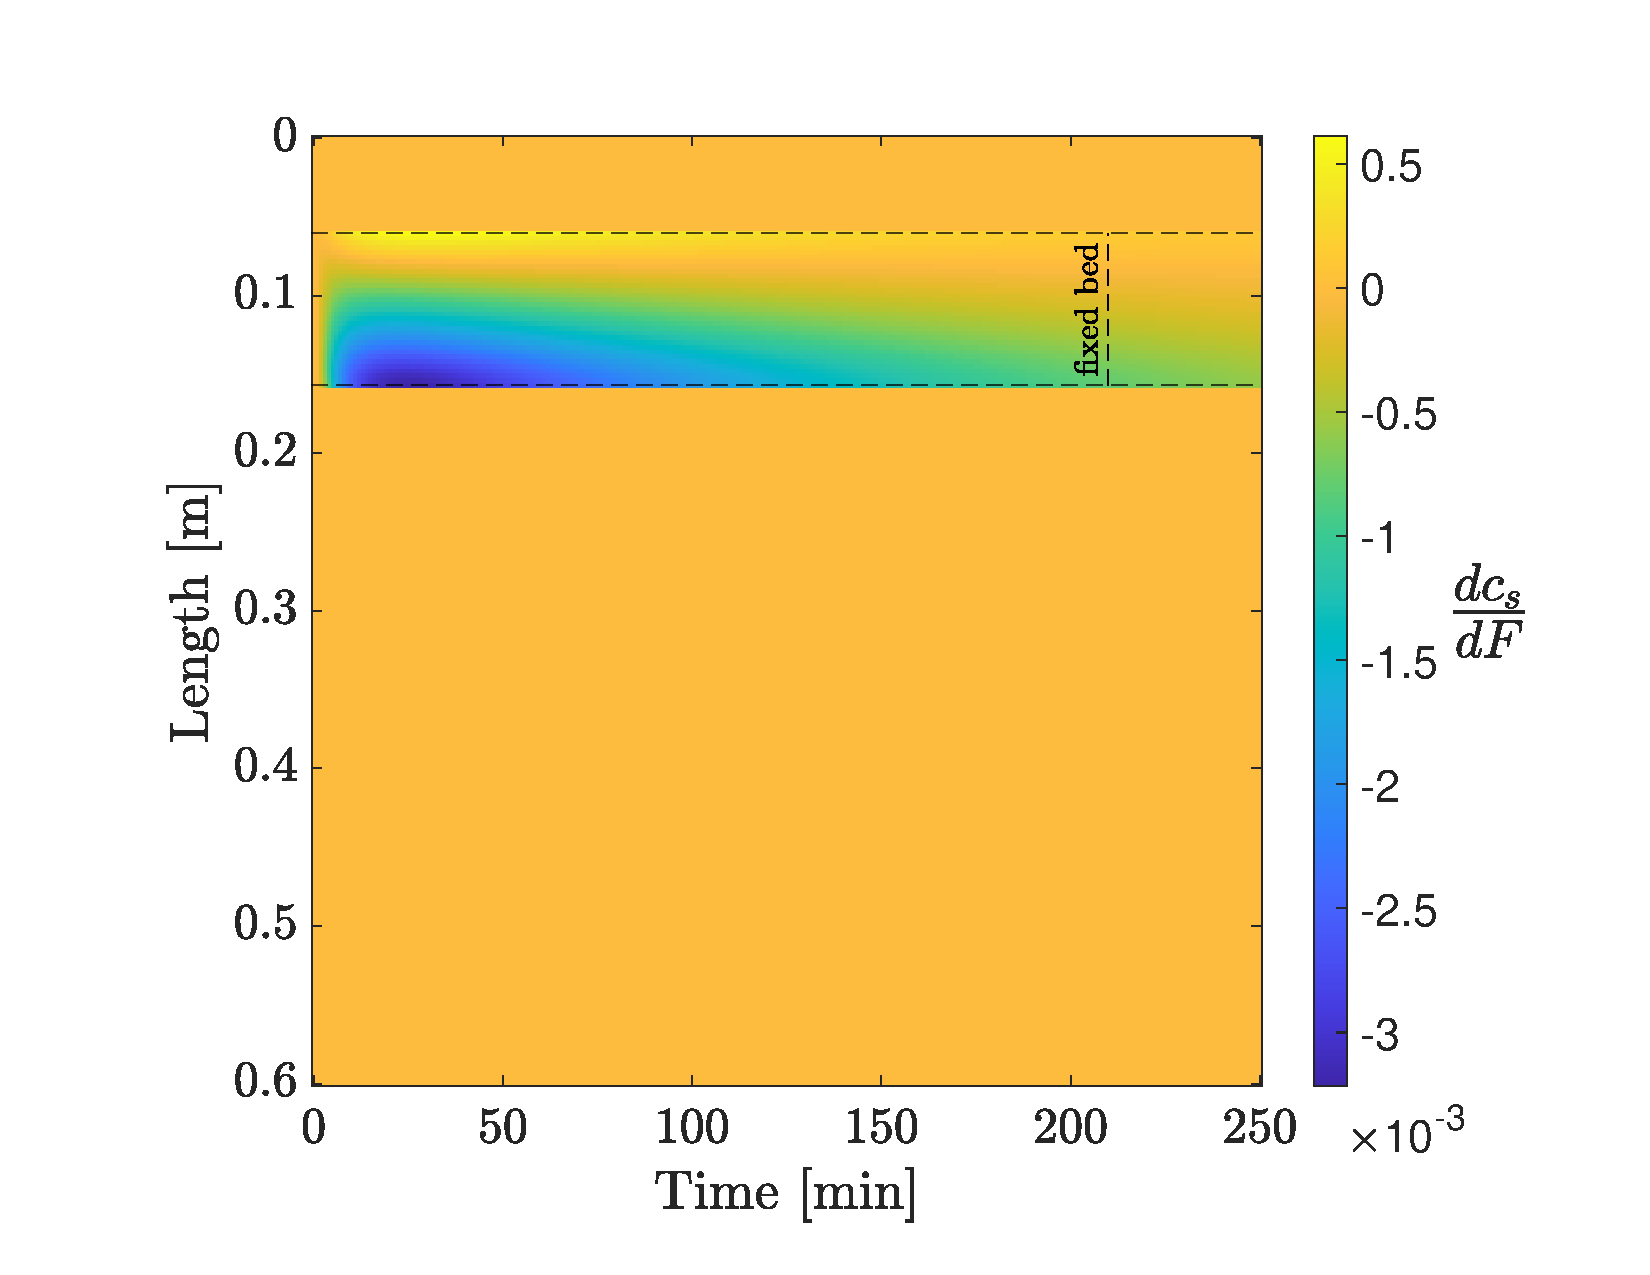
\includegraphics[trim = 1.5cm 1cm 0.5cm 1.0cm,clip,width=\columnwidth]{/Results_sensitivity/CS_F.pdf}
    	\caption{The effect of $F$ change on $C_s$}
    	\label{fig:Sensitivty_F_CS}
    \end{figure}
    
    Figure \ref{fig:Sensitivty_F_CF} shows how the concentration of solute in the fluid phase is affected by the flow-rate increment. Initially, sensitivities are close to zero, which indicates very little system response. The flow-rate growth affects the ${\color{blue}C_f}(z,t)$ by increasing the velocity of the solute across the system, which also increases the concentration gradient. As a result, the positive sensitivities appear in the system and form a front, which moves from the inlet to the outlet of the extractor. Because the larger amount of solute moves faster across the system, the total amount of solute in both phases decreases faster, which eventually causes negative sensitivities to appear in the system. The negative sensitivities form the second front, which moves across the extractor. Eventually, the negative sensitivities asymptotically go to zero.
    
    \begin{figure}[h!]
    	\centering
    	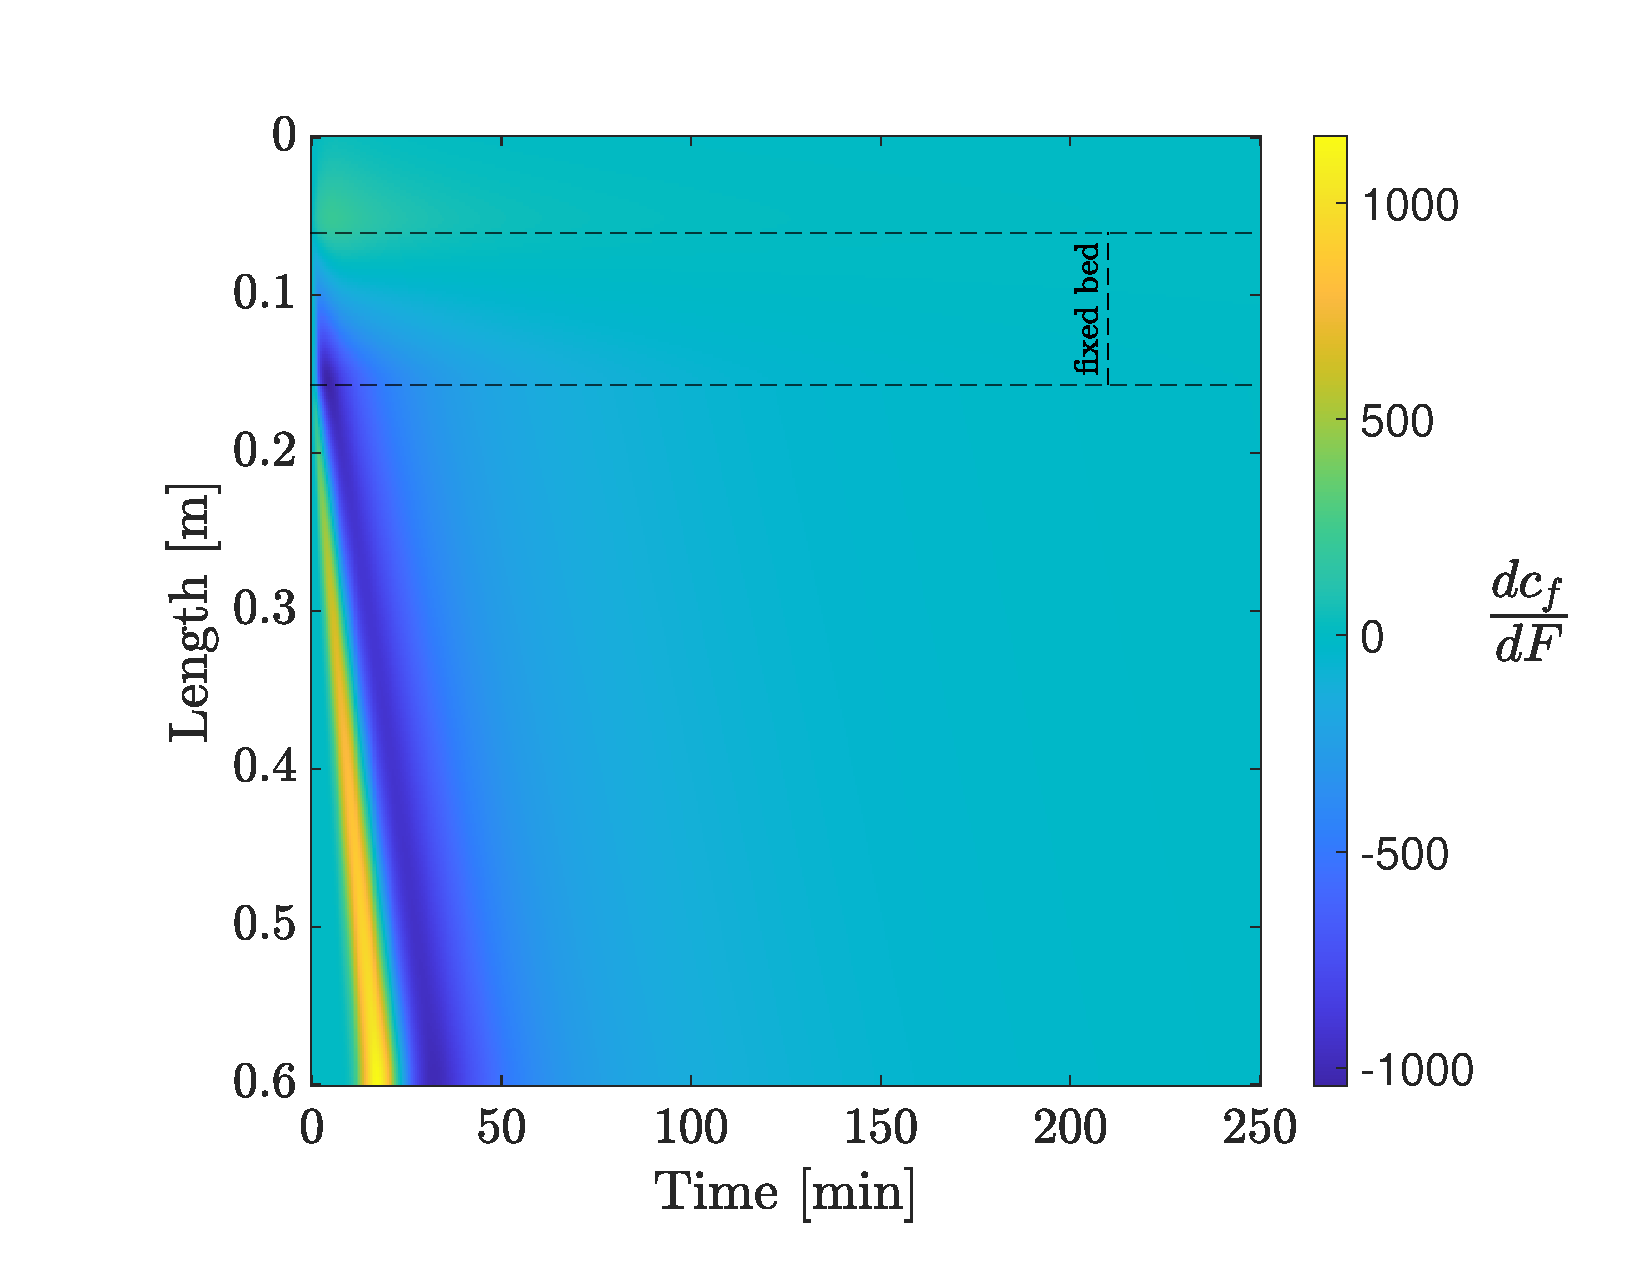
\includegraphics[trim = 1.5cm 1cm 0.5cm 1.0cm,clip,width=\columnwidth]{/Results_sensitivity/CF_F.pdf}
    	\caption{The effect of $F$ change on $C_f$}
    	\label{fig:Sensitivty_F_CF}
    \end{figure}

    Figure \ref{fig:Sensitivty_F_y} shows how the flow-rate increment changes the extraction yield. Initially, the sensitivity curve stays flat, which is caused by the fact that the fixed bed does not occupy the whole volume of the extractor, and the fluid needs some time to flow through the empty part of the extractor to reach its outlet. When the solute in the fluid phase reaches the outlet of the extractor, then system response can be observed. The $dy/dF$ starts to increase, and positive value of sensitivity indicates an improvement in the process efficiency, hence the yield increment. Over time, the sensitivity reaches its maximum and diminishes due to decreasing concentration gradient. The $dy/dF$ asymptotically goes to zero because the amount of solute in the fluid phase becomes a limiting factor of the extraction process, and the flow-rate increment has less effect on the extraction yield. To show how $dy / dF$ converges to zero, the simulation time was expanded.
    
    \begin{figure}[h!]
    	\centering
    	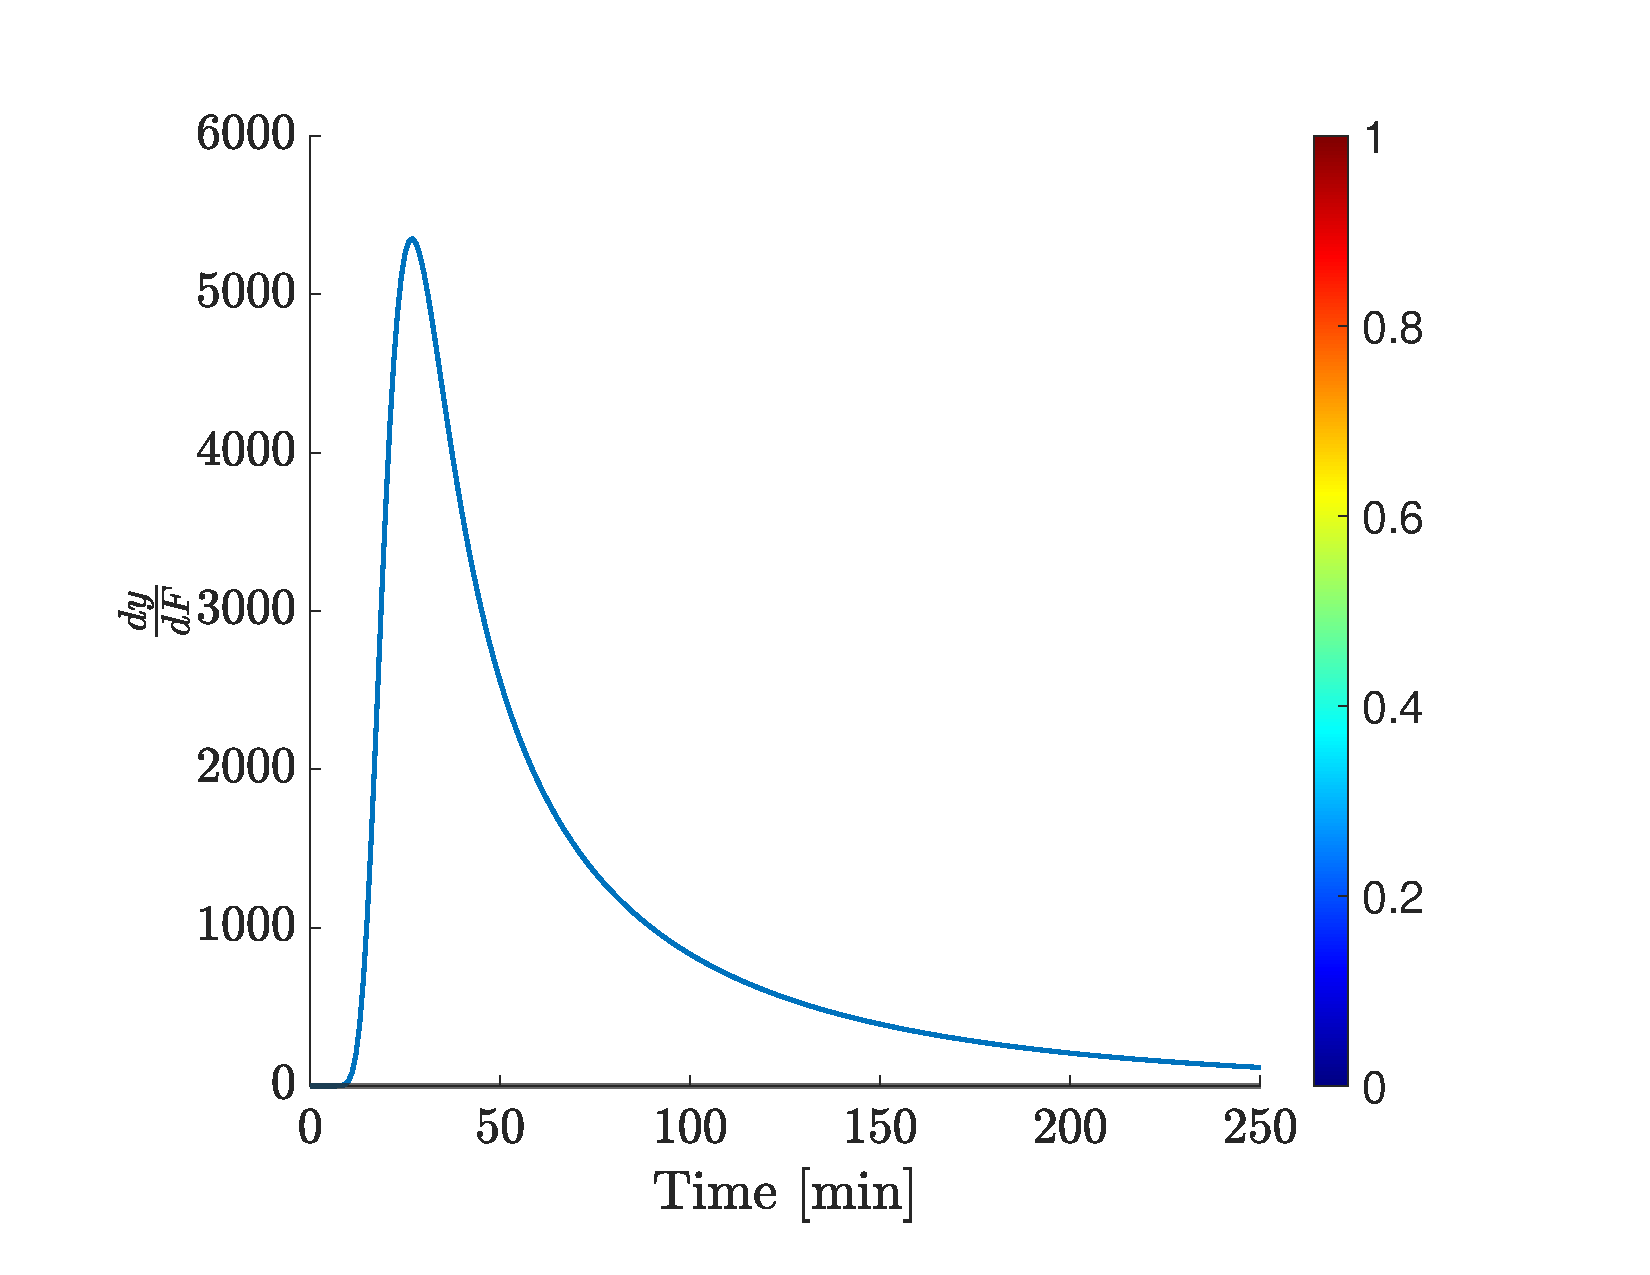
\includegraphics[trim = 1.5cm 1cm 0.8cm 1.0cm,clip,width=\columnwidth]{/Results_sensitivity/Y_F.pdf}
    	\caption{The effect of $F$ change on $y(t)$}
    	\label{fig:Sensitivty_F_y}
    \end{figure}
    
    \subsection{Pressure}
    
    As discussed in Chapter \ref{CH:Governing_equations_chapter}, a small pressure wave propagates with the speed of sound relative to the flow. If the flow velocity is relatively low, all pressure changes are hydrodynamic (due to velocity motion) rather than thermodynamic which leads to $\partial {\color{blue}P}/\partial {\color{orange}\rho_f} = \infty$. The Low Mach-number assumption leads to instant pressure propagation along the system. It allows to consider one value of pressure for the whole system as all the changes occur in the machine simultaneously. Figure \ref{fig:Sensitivty_P_P} represents a step function, which indicate the pressure change in the system. 
    
    \begin{figure}[h!]
    	\centering
    	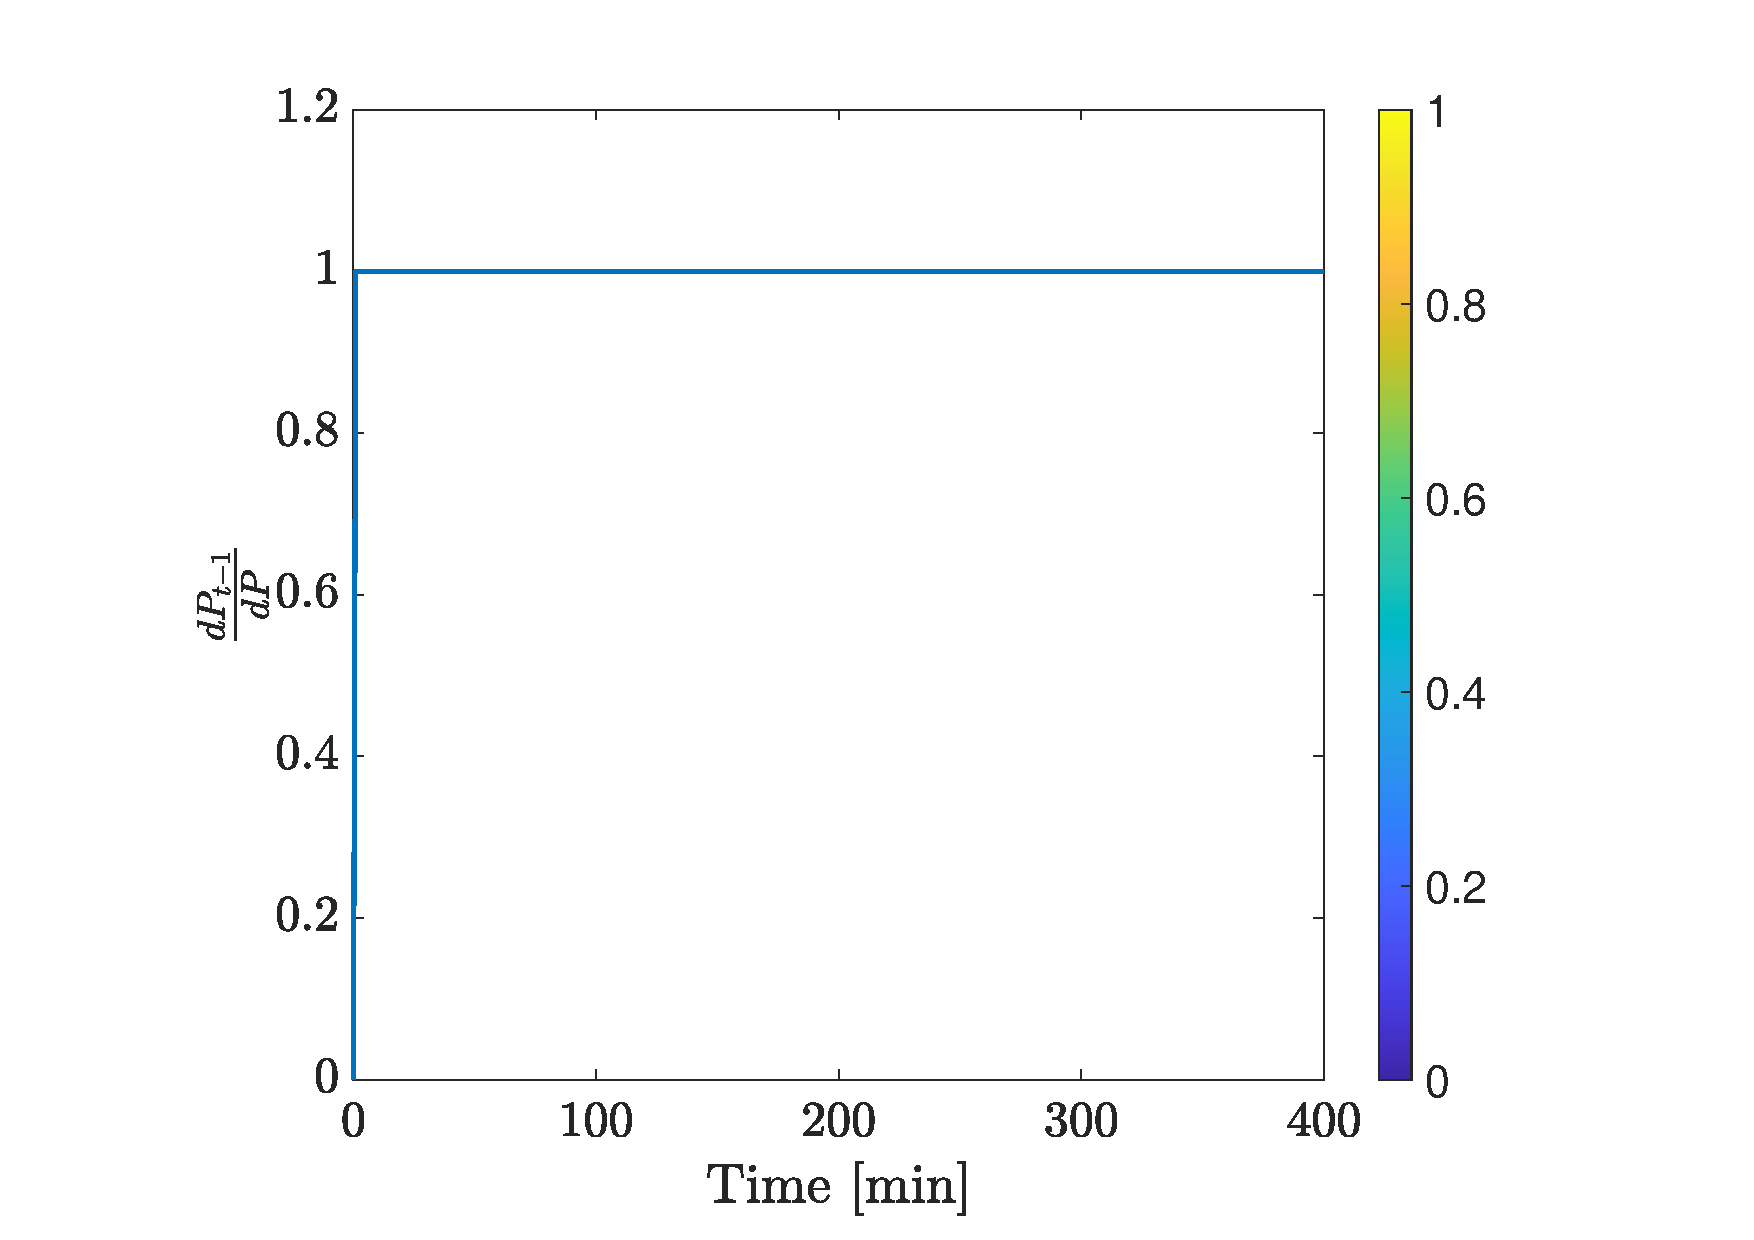
\includegraphics[trim = 1.5cm 1cm 0.8cm 1.0cm,clip,width=\columnwidth]{/Results_sensitivity/P_P.pdf}
    	\caption{The effect of $P$ change on $P$ in the system}
    	\label{fig:Sensitivty_P_P}
    \end{figure}
    
	As a result of the Low Mach-number assumption and the pressure deviation, the temperature and density change along the system simultaneously. According to Equation \ref{EQ:Enthalpy_equation}, the pressure change affect the quantity $h \times \rho_f$ directly through $\partial ({\color{blue}P}(t) A_f) / \partial t$, which leads to a step-change presented in Figure \ref{fig:Sensitivty_P_H}. Depending on the configuration of the system, two cases are possible. As the total energy in the extractor has changed, there might be a difference between the fluid inside the equipment and the inlet temperature(defined as a boundary condition). If the Dirichlet boundary condition is applied, the inlet temperature is kept at the pre-defined value and might differ from the temperature in the extractor. In such a case, the temperature difference will cause the heat front to propagate through the system. Alternatively, the Neumann boundary condition can be applied to ensure that the temperature inside the extractor and at its inlet is the same. In the case of this work, the second approach was chosen to simplify the discussion.
    
    \begin{figure}[h!]
    	\centering
    	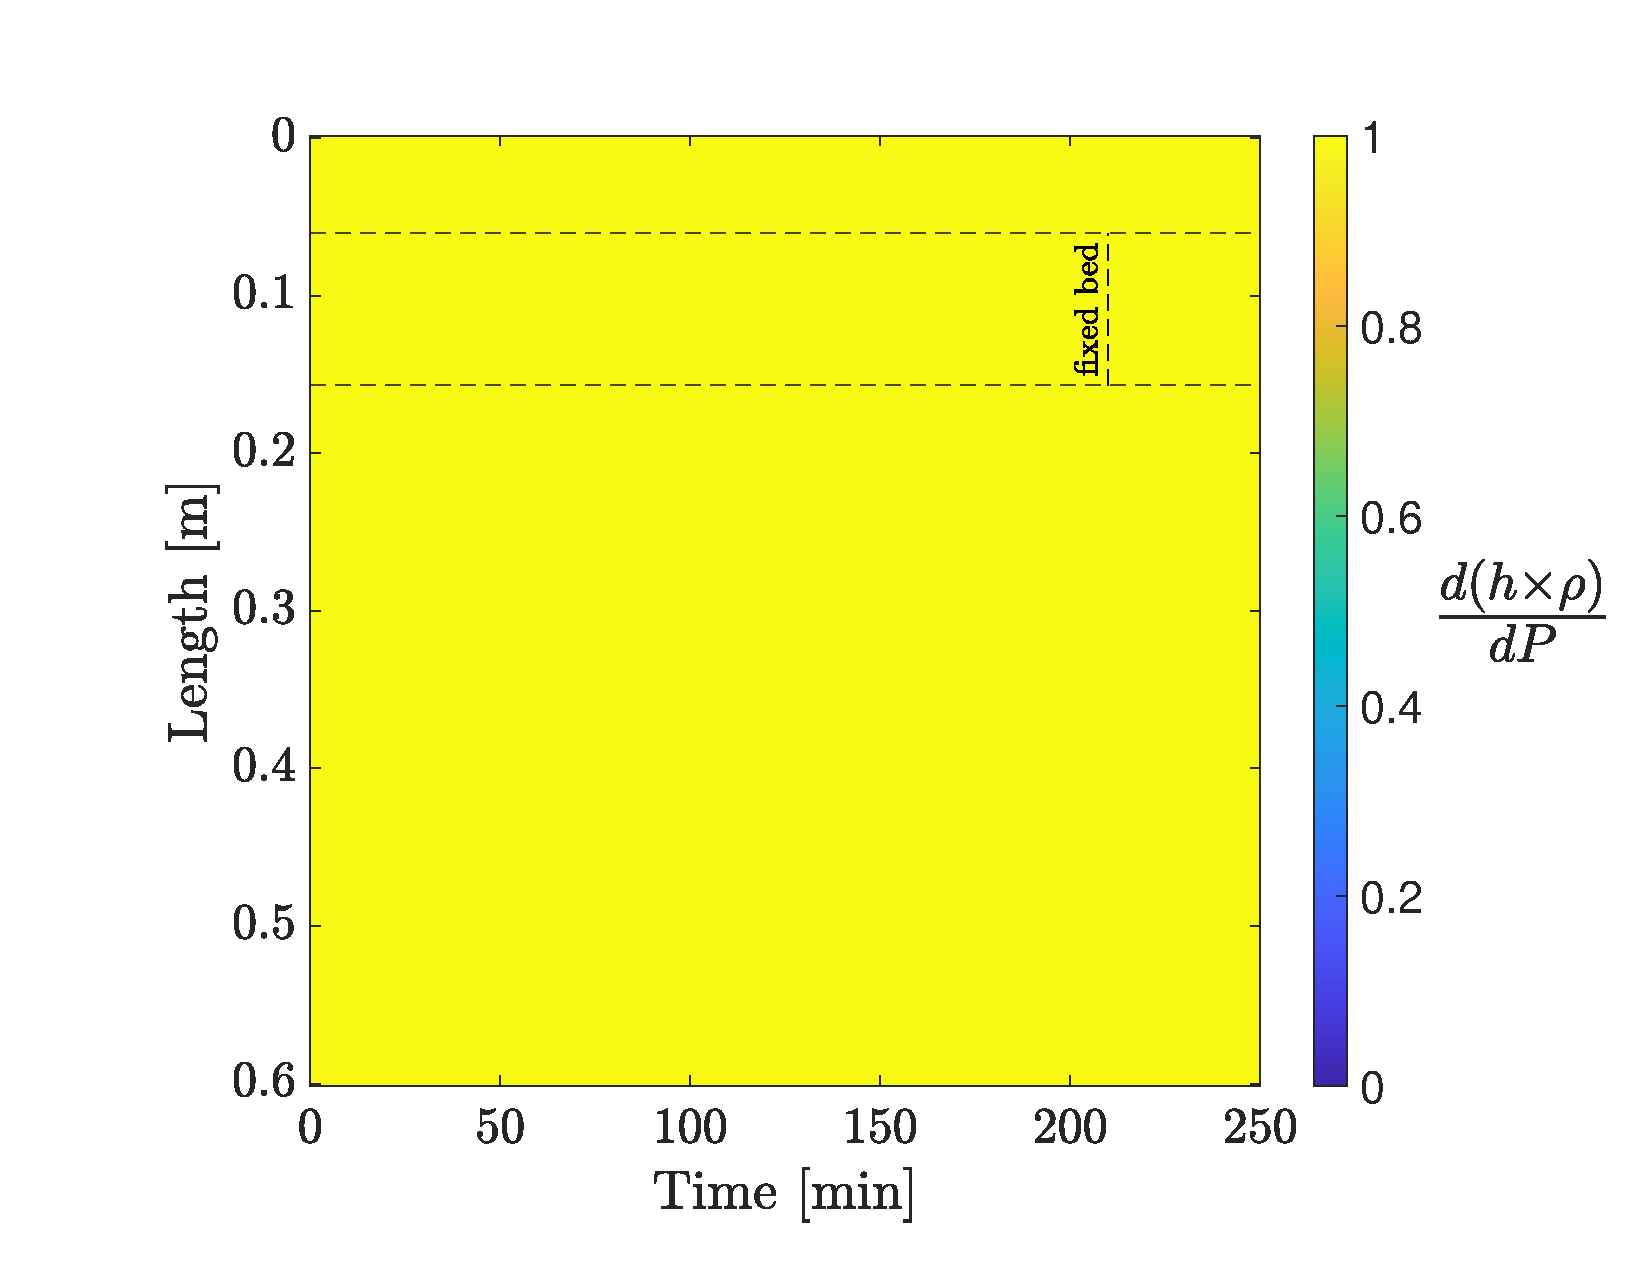
\includegraphics[trim = 1.5cm 1cm 0.8cm 1.0cm,clip,width=\columnwidth]{/Results_sensitivity/H_P.pdf}
    	\caption{The effect of $P$ change on $(h \times \rho_f)$ in the system}
    	\label{fig:Sensitivty_P_H}
    \end{figure}

	The pressure change affects the mass transfer in two ways. As given in Chapter \ref{CH: Continuity}, the velocity is inversely proportional to the density; hence, the higher density of the fluid leads to a lower velocity and larger residence time. The second way is given by the relationships, which connect the pressure and the extraction kinetic term. As presented in {\color{red}article 1}, the $D_i^R$ increases with the fluid density, which leads to a higher extraction rate. The cumulative effect of the pressure change can be observed in Figure \ref{fig:Sensitivty_P_CS}. The sensitivity plot shows a uniform decay of sensitivities along the fixed bed. The negative values of sensitivities suggest a faster extraction rate. No matter the location of the sensitivity in the bed, the general behaviour stays the same. Every sensitivity starts with zero and decreases to a minimum value. After the extremum, the sensitivities asymptotically increase to zero.

	\begin{figure}[h!]
		\centering
		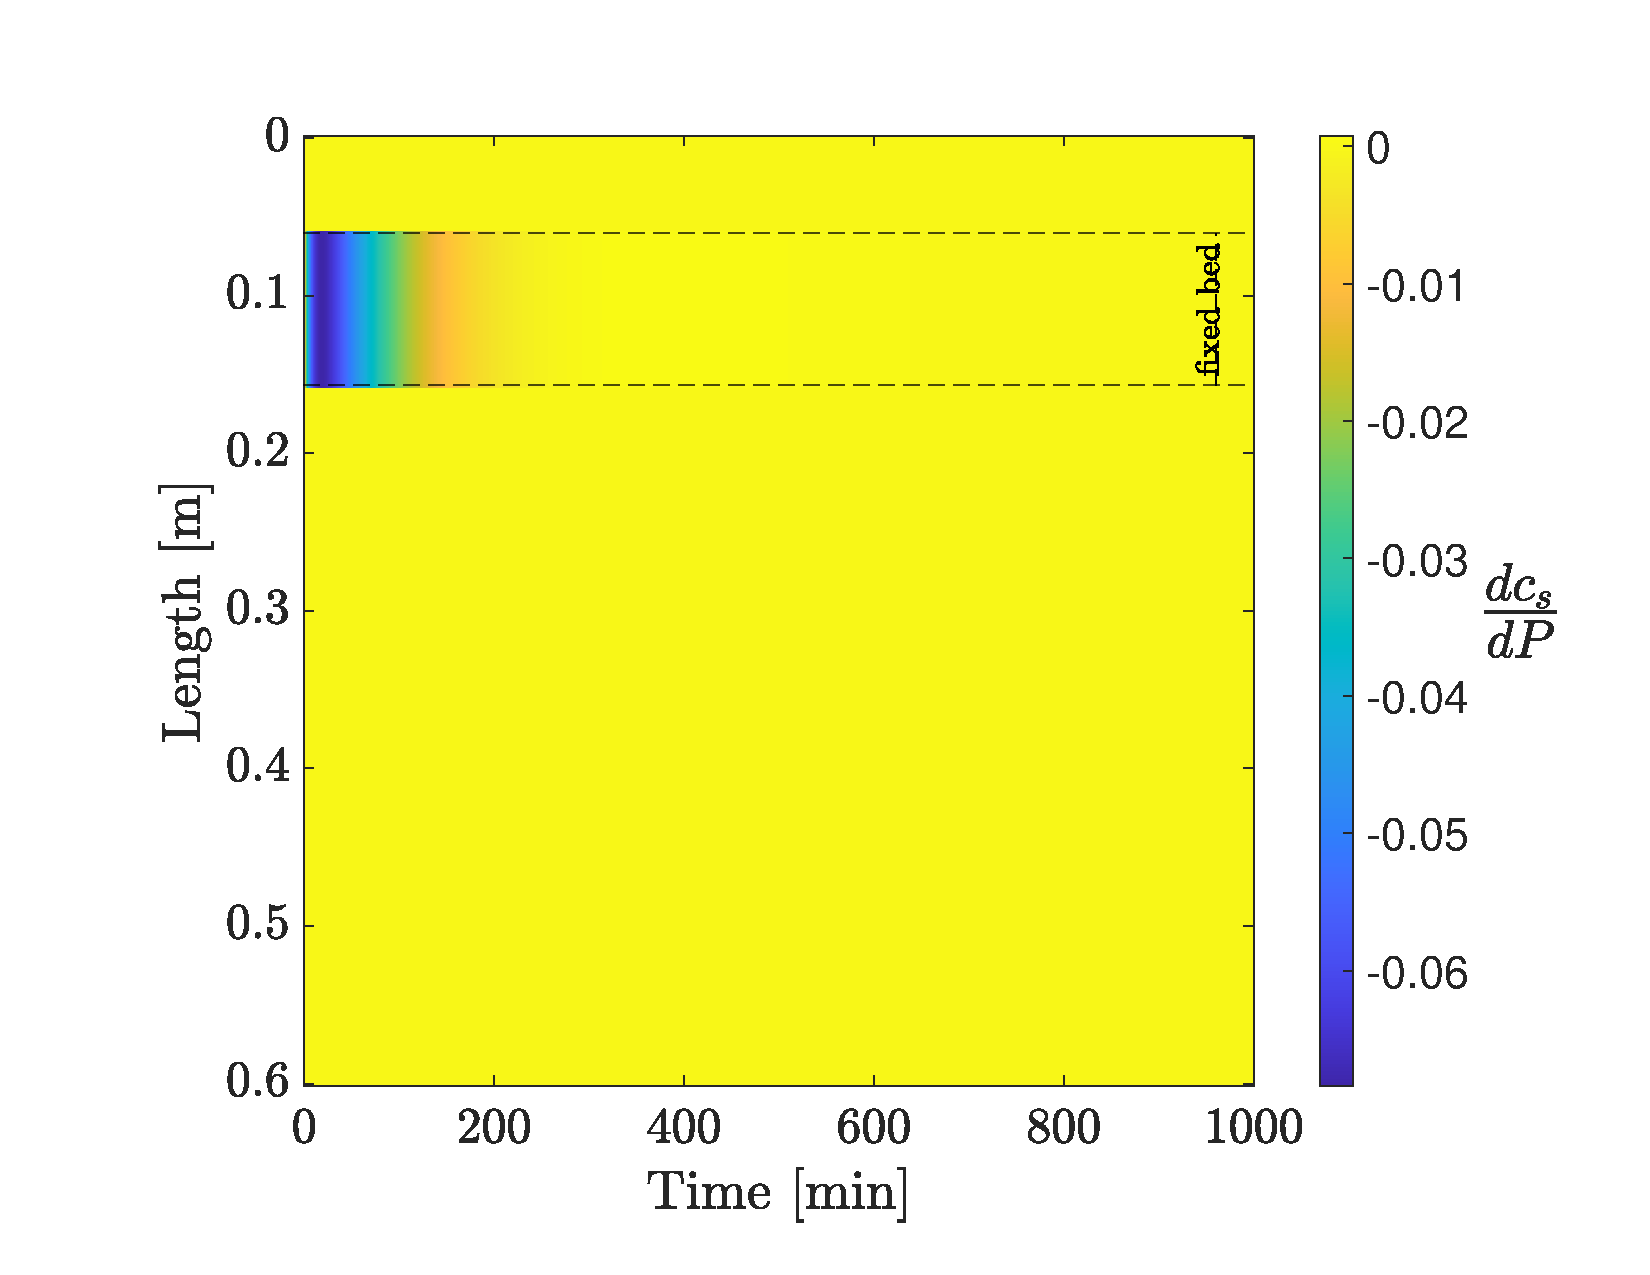
\includegraphics[trim = 1.5cm 1cm 0.8cm 1.0cm,clip,width=\columnwidth]{/Results_sensitivity/CS_P.pdf}
		\caption{The effect of $P$ change on $C_s$}
		\label{fig:Sensitivty_P_CS}
	\end{figure}

	The corresponding response of the pressure change on the solute concentration in the fluid phase is presented in Figure \ref{fig:Sensitivty_P_CF}. As discussed above, the pressure change directly affects the extraction kinetics. Figure \ref{fig:Sensitivty_P_CS} is characterized by negative sensitivities, which suggest a higher extraction rate due to pressure change. It is expected to observe an increase of solute in the fluid phase due to a higher extraction rate. That increase of the solute in the fluid phase is visible in Figure \ref{fig:Sensitivty_P_CF} as positive sensitivities, which forms a front moving along the extractor. As the extraction is faster, more solute goes to the fluid phase, explaining the hot spot in the Figure. Then, the solute flows along the system, where there are no solid particles, and the diffusion effect becomes noticeable. After the positive sensitivities, a small front of negative sensitivities can be observed. Due to higher extraction rate, more solute has been extracted at the beginning of the extraction time, which means that there is less solute to extract later, and that effect is visible in Figure \ref{fig:Sensitivty_P_CF} as a negative sensitivities.

	\begin{figure}[h!]
		\centering
		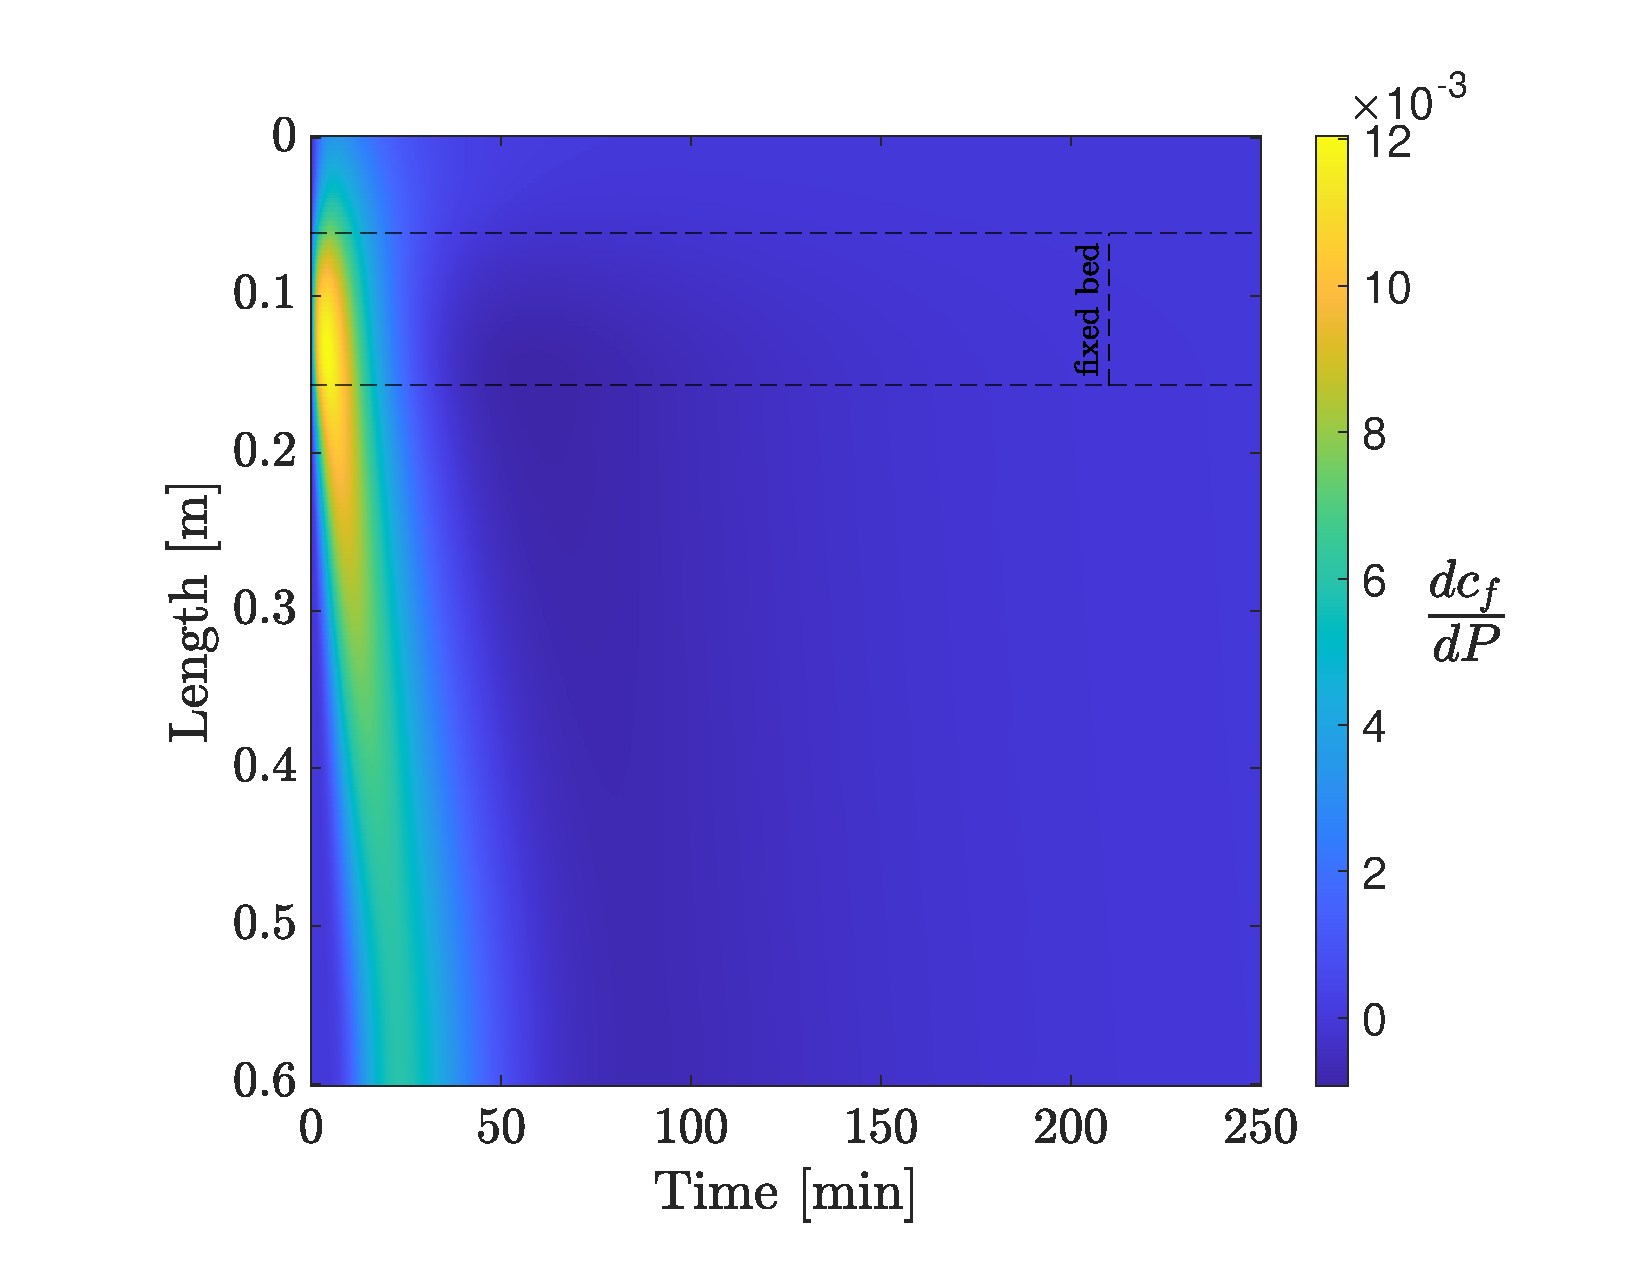
\includegraphics[trim = 1.5cm 1cm 0.8cm 1.0cm,clip,width=\columnwidth]{/Results_sensitivity/CF_P.pdf}
		\caption{The effect of $P$ change on $C_f$}
		\label{fig:Sensitivty_P_CF}
	\end{figure}

	The effect of the pressure increase on the extraction yield is presented in Figure \ref{fig:Sensitivty_P_y}. The initial flat curve is related to a delay in the system caused by empty space in the extractor, through which the solvent with solute needs to flow to reach the outlet. Later, the positive sensitivity is present and indicates an increase in yield. The $dy / dP$ reaches a maximum and starts to decrease due to the lower amount of the solute left in the solid phase compared with the case before the pressure increment. The sensitivity decreases to negative values, reaches a minimum, and eventually goes zero. To show how $dy / dP$ converges to zero, the simulation time was expanded.

	\begin{figure}[h!]
		\centering
		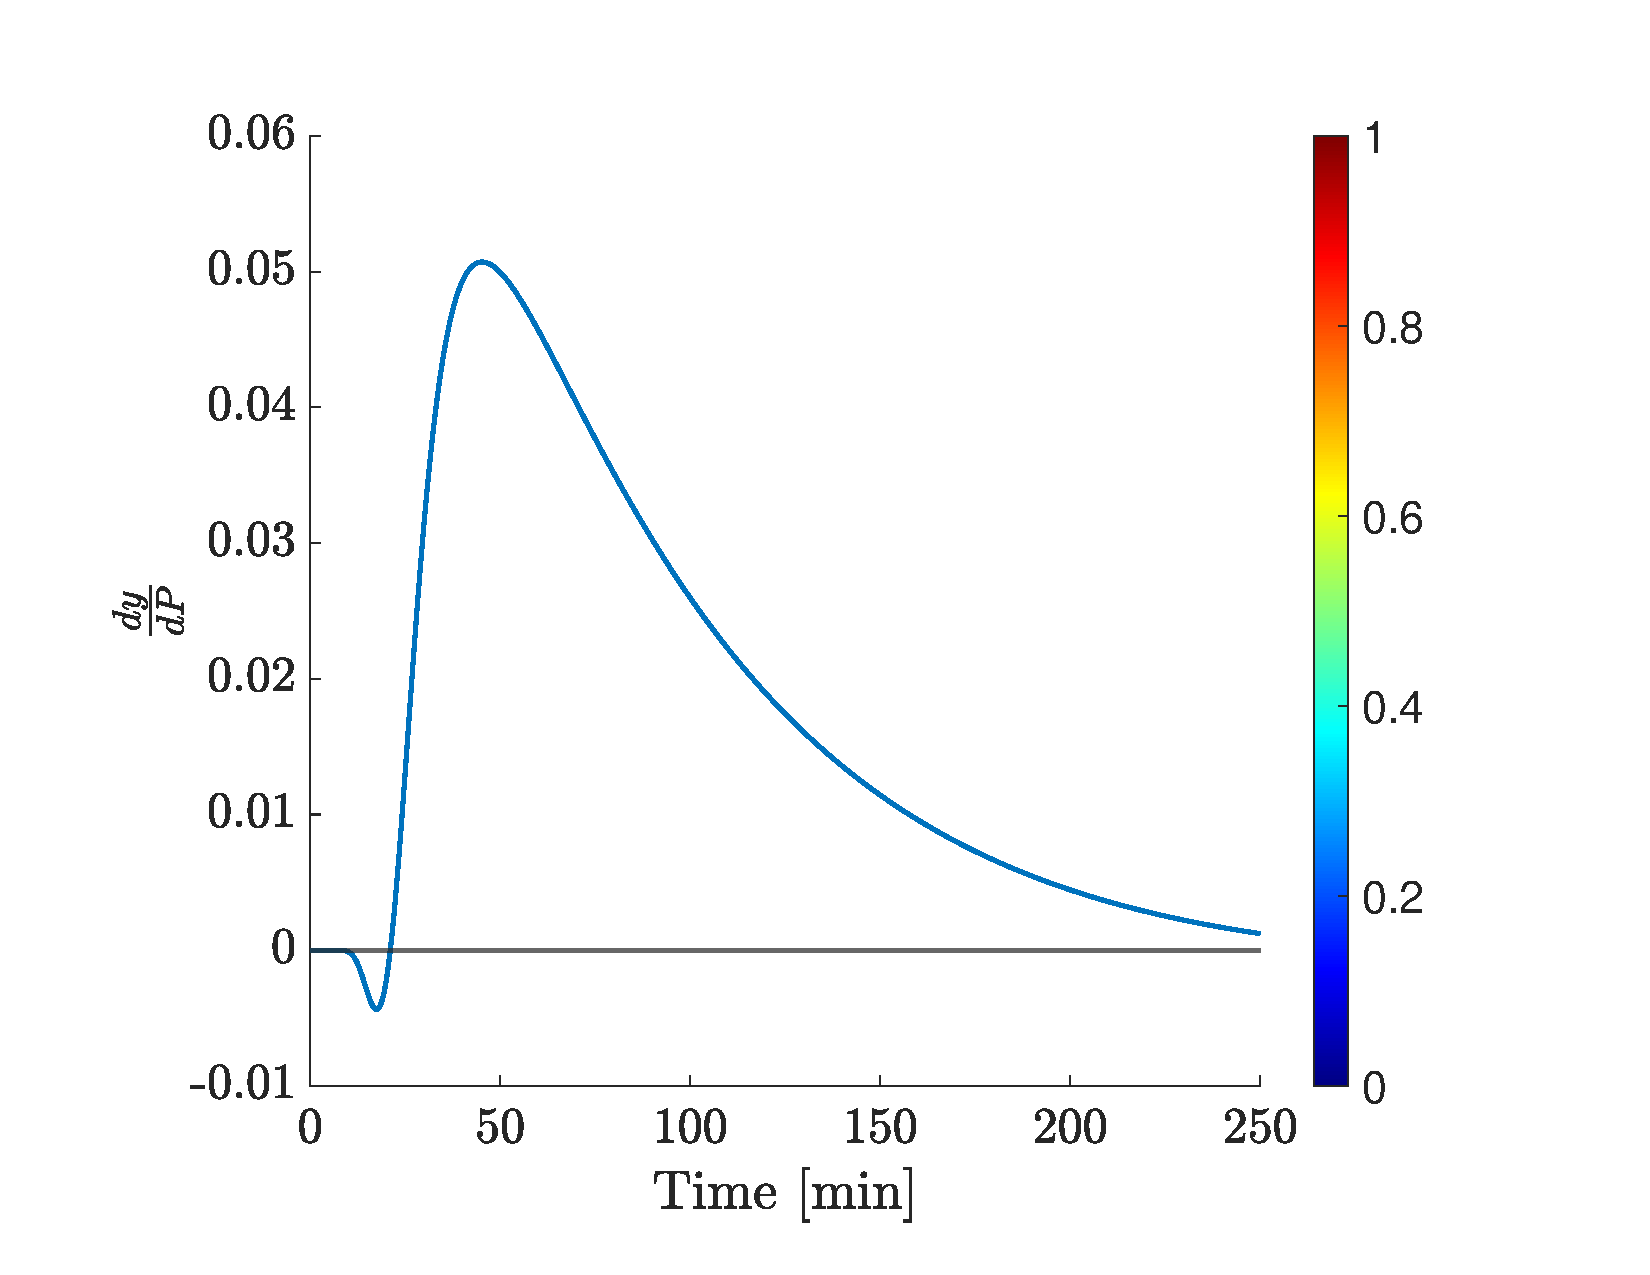
\includegraphics[trim = 1.5cm 1cm 0.8cm 1.0cm,clip,width=\columnwidth]{/Results_sensitivity/Y_P.pdf}
		\caption{The effect of $P$ change on $y(t)$}
		\label{fig:Sensitivty_P_y}
	\end{figure}

	\subsection{Inlet temperature}
	
	The influence of the inlet temperature on the supercritical extraction differs from the two presented cases because the disturbance does not affect the whole system instantaneously but propagates through the system. As the fluid with modified temperature flows along the system, it gradually affects the mass transfer. One assumption is that inlet temperature does not affect the pressure, and because of that, a horizontal line is present in Figure \ref{fig:Sensitivty_P_T}.
	
	\begin{figure}[h!]
		\centering
		\includegraphics[trim = 1.5cm 1cm 0.8cm 1.0cm,clip,width=\columnwidth]{/Results_sensitivity/P_T_{in}.pdf}
		\caption{The effect of $T_{in}$ change on $P$ in the system}
		\label{fig:Sensitivty_P_T}
	\end{figure}

	The propagation of the heat front is presented in Figure \ref{fig:Sensitivty_T_H}. The inlet value of $(h\times \rho_f)$ is calculated based on the given value of the inlet temperature( Dirichlet boundary condition) and given pressure. The deviation in $T_{in}$ affects $(h\times \rho_f)$ at the inlet, which propagates according to the governing equations. 
	
	\begin{figure}[h!]
		\centering
		\includegraphics[trim = 1.5cm 1cm 0.8cm 1.0cm,clip,width=\columnwidth]{/Results_sensitivity/H_T_{in}.pdf}
		\caption{The effect of $T_{in}$ change on $(h \times \rho_f)$ in the system}
		\label{fig:Sensitivty_T_H}
	\end{figure}

	Figure \ref{fig:Sensitivty_T_CS} shows how the concentration of the solute in the solid phase is affected by the inlet temperature change. Initially, the sensitivities are zero along the fixed bed because the heat front needs time to propagate to the fixed bed. As the propagation is not instantaneous, the non-uniform distribution of sensitivities along the fixed bed is visible. All the sensitivities start to grow and reach maxima. As presented in {\color{red}article 1}, the value of $D_i^R$ diminishes when the density decreases. It is expected to observe positive sensitivities in Figure \ref{fig:Sensitivty_T_CS}, which indicates a slower extraction rate. When the concentration gradient becomes a limiting factor, the sensitivities decrease.

	\begin{figure}[h!]
		\centering
		\includegraphics[trim = 1.5cm 1cm 0.8cm 1.0cm,clip,width=\columnwidth]{/Results_sensitivity/CS_T_{in}.pdf}
		\caption{The effect of $T_{in}$ change on $C_s$ in the system}
		\label{fig:Sensitivty_T_CS}
	\end{figure}

	The influence of the inlet temperature on the solute in the fluid phase is shown in Figure \ref{fig:Sensitivty_T_CF}. At the start, all the sensitivities stay at zero because of idle time. When the fluid at a new temperature reaches the solid particles, it affects the mass transfer, which later affects the amount of the solute in the fluid phase. As a response to the slower extraction rate suggested by positive sensitivities in Figure \ref{fig:Sensitivty_T_CS}, the 'hot spot' with negative sensitivities is visible in Figure \ref{fig:Sensitivty_T_CF}. An effect of the diffusion can be observed in the section without the fixed bed where the front made of sensitivities becomes blurry. After the sensitivities reach minima, they grow and reach positive values. This behavior can be explained by considering that the heat front slowed the mass transfer, and more of the solute stayed in the solid phase. That leads to a higher concentration gradient in the later time of the extraction if compared to the situation without the inlet temperature deviation. The higher concentration gradient causes the increase of the $dc_f/dT_{in}$.
	
	\begin{figure}[h!]
		\centering
		\includegraphics[trim = 1.5cm 1cm 0.8cm 1.0cm,clip,width=\columnwidth]{/Results_sensitivity/CF_T_{in}.pdf}
		\caption{The effect of $T_{in}$ change on $C_f$ in the system}
		\label{fig:Sensitivty_T_CF}
	\end{figure}

	Figure \ref{fig:Sensitivty_T_y} shows how the inlet temperature increment changes the extraction yield. Initially, the sensitivity curve stays flat, which is caused by the fact that the fixed bed does not occupy the whole volume of the extractor, and the fluid needs some time to flow through the empty part of the extractor to reach its outlet. When the solute in the fluid phase reaches the outlet of the extractor, then system response can be observed. The $dy/dT_{in}$ starts to decrease, and the negative sensitivity value indicates a worsened process efficiency. Over time, the sensitivity reaches its minimum and increases due to a higher concentration gradient (if compared to the case without the disturbance). The sensitivity reaches a positive maximum and decreases again due to lower reduced extraction kinetic and decreased concentration gradient. The $dy/dT_{in}$ becomes negative again, and eventually the sensitivity curve flattens.

	\begin{figure}[h!]
		\centering
		\includegraphics[trim = 1.5cm 1cm 0.8cm 1.0cm,clip,width=\columnwidth]{/Results_sensitivity/Y_T_{in}.pdf}
		\caption{The effect of $T_{in}$ change on $y(t)$ in the system}
		\label{fig:Sensitivty_T_y}
	\end{figure}
	
\end{document}


































